\documentclass{article}
\usepackage{url,graphicx,amssymb,array}
\usepackage[savemem]{listings} 
\usepackage{lstpatch,lstomdoc}
\usepackage[hide]{draftstamp,ed} %set this to [hide] in the final version
\usepackage[hide]{xmlindex}
\usepackage{svn}
\usepackage{wrapfig}
\makeindex
%\SVN $Id: mkm06.tex 7947 2006-05-24 13:31:40Z kohlhase $
%\SVNdate $Date: 2006-05-24 15:31:40 +0200 (Wed, 24 May 2006) $

\def\chemml{{\sc{CML}}}
\def\physml{{\sc{PhysML}}}
\def\stex{{\raisebox{-.5ex}S\kern-.5ex\TeX}}
\def\om#1{\fbox{\ensuremath{#1}}}
\lstset{float=htb,columns=flexible,frame=lines,language=[omdoc]XML,basicstyle=\scriptsize,
  indexstyle=\indextt,indexstyle=[1]\indexelement,indexstyle=[2]\indexattribute,showstringspaces=false}

%% to number the listings in sequence with figures
\makeatletter\let\c@lstlisting\c@figure\makeatother

\def\LNAI{LNAI}
\def\LNCS{LNCS}
\def\PROC{Proceedings }
\def\cG{{\cal G}}

\def\google{\sc{Google}}
\def\googlescholar{\sc{Google Scho\-lar}}
\def\mathematica{\sc{Mathematica}}
\def\gap{\sc{Gap}}
\def\wikipedia{\sc{Wiki\-Pedia}}
\def\soap{\sc{Soap}}
\def\owl{\sc{Owl}}

\def\deq{\colon=}
\def\defin#1{{\bf{#1}}}
\def\name#1{{{\small{\sc{#1}}}}}
\def\seen{seen }
\def\July{July }
\def\webpageat{Web page at }
\def\mathml{\sc{MathML}}
\def\openmath{\sc{OpenMath}}
\def\omdoc{\sc{OMDoc}}
\newenvironment{myfig}[2]%
{\begin{figure}[!htb]\def\myfiglabel{#1}\def\myfigcaption{{#2}}\begin{center}}
{\caption{\myfigcaption}\label{fig:\myfiglabel}\end{center}\vspace{-2em}\end{figure}}

\def\myfigref#1{Figure~\ref{fig:#1}}
\def\myfigsref#1#2{Figures~\ref{fig:#1} and~\ref{fig:#2}}
\def\myfiglref#1#2{Figures~\ref{fig:#1} to~\ref{fig:#2}}
\def\Myfigref#1{Figure~\ref{fig:#1}}  % this one is capitalized for sentence beginnings

\title{}
\author{Eberhard Hilf \\
Institute for Science Networking, Oldenburg\\
  \url{hilf@isn-oldenburg.de}\\[.5cm]
Michael Kohlhase\\
  Computer Science, International University Bremen\\
  \url{m.kohlhase@iu-bremen.de}\\[.5cm]
Heinrich Stamerjohanns\\
  Computer Science, International University Bremen\\
  \url{h.stamerjohanns@iu-bremen.de}}

\begin{document}
\hyphenation{veri-fied
        }

\maketitle

\begin{center}\textit{SVN Id: \SVNId}\end{center}

\begin{abstract}
  We present a content markup language for physics realized by extending the {\omdoc}
  format by an infrastructure for the principal concepts of physics: {\emph{observables}},
  physical {\emph{systems}}, and {\emph{experiments}}. The formalization of the
  description of physics observables follows the structural essence of the operational
  theory of physics measurements. The representational infrastructure for systems and
  experiments allow to capture the distinctive practice of physics: natural laws are
  supported by evidence from experiments which are described, disseminated and reproduced
  by others.
\end{abstract}

\setcounter{tocdepth}{3}\tableofcontents\newpage

\section{Introduction}\label{sec:intro}

The distributivity of information and services over the Internet has changed all aspects
of life, and science is not an exception. We anticipate that the systems currently
investigated in the community will eventually change scientific practice and that they
will have a strong societal impact, provided that they can inter-operate to cover the
whole work-flow of scientific research, education and application. 
\begin{wrapfigure}{r}{6.5cm}\vspace{-.6cm}
  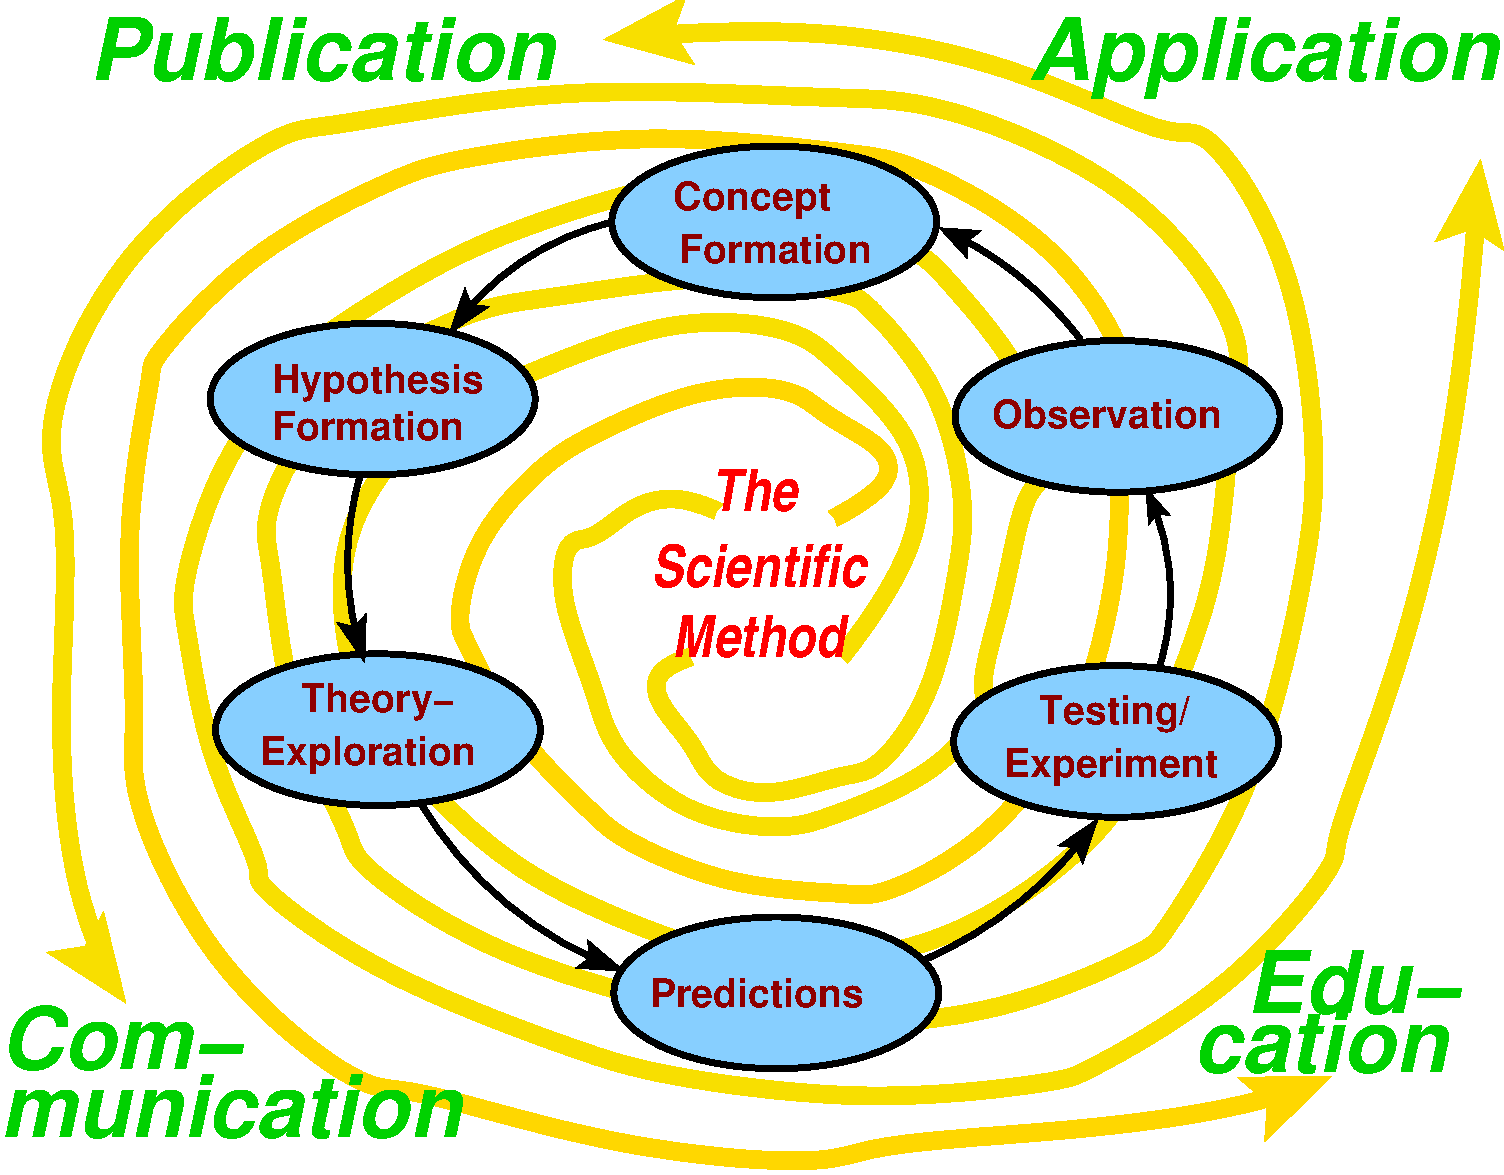
\includegraphics[width=6.5cm]{sci-method}\vspace{-.3cm}
  \caption{The Scientific Method}\label{fig:nw-Methode}\vspace{-.6cm}
\end{wrapfigure}
To further this vision we need to develop, implement, and provide semantic-based and
context-aware techniques for acquiring, organizing, processing, sharing and using
knowledge in science.
 
Our starting point is the view of the {\emph{scientific method}} as a spiral (see
Fig.~\ref{fig:nw-Methode}), where we have our focus on physics here.  In this view,
scientific research in physics moves in a spiral trajectory from original ideas to results
and even applications. Ideas pass through the processes of observation of natural
processes, then of concept formulation to describe these. These allow scientists to
express initial theories about (quantitative laws of nature governing) them, which are
then explored (what are the consequences of the model assumptions) leading to predictions
about processes that can be verified or falsified (to a certain degree) experimentally.
These experiments usually lead to new observations, starting the next round in the spiral
until a quantitative (mathematically formulated) \textit{theory} predicting exclusively
correct results from experiments is formulated.  Observables in physics have to be
suitably found such that they can be physically measured, their algebraic counterparts
being then candidates for building stones of a theory.  The semantics of mathematics as
such is more confined, searching for logically correct sets of rules.

At the moment, most of the steps in Fig.~\ref{fig:nw-Methode} are separately supported by
software systems, e.g.  literature searches in {\googlescholar} or {\wikipedia}, theory
exploration in computer algebra systems like {\mathematica}, and experiments in simulation
systems. But the systems are, by and large, not able to inter-operate since they use
differing data formats, make differing model assumptions, and are bound to an implicitly
given context that is only documented in publications about the systems. For instance,
copy-and-paste from {\googlescholar} or {\wikipedia} to {\mathematica} or a simulation
system is impossible because of this format problem. Moreover, where possible, copy and
paste can be very dangerous, since computer algebra systems make differing assumptions on
the Computercode-libraries, 
the simulation systems are based on\footnote{A simple example, where the lack of
explicit context led to a very expensive failure was the September 1999 loss of a \$125
million Mars orbiter, which crashed on Mars. The cause was that NASA used for its
specifications metric units, but the Lockheed Martin engineers misinterpreted the data
assuming they were given using Imperial units of measurement.}.

We are set here to arrive at a content markup format for physics. Early concept
discussions and visions~\cite{Hilf:texdocc,PML:web,Hilf:guestrow,Hilf:p05} have not led to
a realization in terms of an encoding, since the problem was attacked from the ground up.
In this paper we will build the bridge from vision to a usable markup language by
extending the {\omdoc} ({\underline{O}pen} {\underline{M}athematical}
{\underline{Doc}uments}) format~\cite{Kohlhase:omdoc1.2} by an infrastructure for
(physical) systems, observables and experiments and call this new module and the extended
system {\physml} (Physics Markup Language). Since we can now share all the infrastructure
--- in particular the theory and statement levels --- with mathematics, the language
design for {\physml} becomes feasible.


%%% Local Variables: 
%%% mode: stex
%%% TeX-master: "mkm06"
%%% End: 

% LocalWords:  cience ech logy ngineering athematical uments ciences echnology
% LocalWords:  athematics stex mkm

%%
%% This file generates files required to use the ed package.
%% At your command prompt write
%%
%%     latex physml.ins
%%
%% Copyright(c) 2008 Michael Kohlhase
%%
%% This file is distributed under the terms of the LaTeX Project Public
%% License from CTAN archives in directory  macros/latex/base/lppl.txt.
%% Either version 1.0 or, at your option, any later version.
%%
\input docstrip
\preamble
\endpreamble

%\usedir{tex/latex/listings}
\keepsilent
\askforoverwritefalse

% generate base package
\generate{\file{physml.sty}{\from{physml.dtx}{package}}}

\Msg{*}
\Msg{* You probably need to move the generated style files into a directory searched by TeX.}
\Msg{*}
\Msg{* And don't forget to refresh your filename database}
\Msg{* if your TeX distribution uses such a database.}
\Msg{*}

\nopreamble\nopostamble
\generate{\file{physml.sty.ltxml}{\from{physml.dtx}{ltxml}}}

\Msg{*}
\Msg{* You probably need to move the generated ltxml files into a directory searched by LaTeXML.}
\Msg{*}

\endbatchfile

\def\llquote#1{\ensuremath{\langle\kern-.25em\langle{#1}\rangle\kern-.25em\rangle}}
\def\PHYSmodule#1{\module{PHYS}{#1}{Foundations of Physics}} 
\def\mobjabbr{OMOBJ |m:math |legacy}
\def\module#1#2#3{#1}
\def\indextoo#1{#1}
\def\snippet#1{\tt{#1}}
\def\Kelvin{K}
\def\Celsius{{}^{\circ}C}

\section{Extending OMDoc for Physics}\label{HandleOnKnowledge}

In this section we will extend the {\omdoc} format\footnote{Due to space restrictions we
  cannot introduce the format here; we refer the reader to~\cite{Kohlhase:omdoc1.2} for
  the language definition and examples.} by an infrastructure for (physical) systems,
observables and experiments.
\begin{figure}
\begin{center}\scriptsize
\begin{tabular}{|>{\tt}l|>{\tt}l|>{\tt}l|>{\tt}p{5.5cm}|}\hline
{\rm Element}& \multicolumn{2}{l|}{Attributes} & Content  \\\hline
             & {\rm Req.}  & {\rm Optional}     &           \\\hline\hline
 observable  & name & algebra, xref & metadata?, opdef, refinement, type?\\\hline
 refinement  &      & xml:id, xref & metadata?, CMP*, FMP*\\\hline 
 opdef       &      & xml:id, xerf & metadata?, CMP*, FMP*\\\hline\hline
 system      &     & xml:id, xref & metadata?, realization?, observable*, 
                                               preparation?, state?\\\hline
 realization &     & xml:id & metadata?, CMP*, FMP*\\\hline 
 preparation &     & xml:id & metadata?, CMP*, FMP*\\\hline 
 state       & of  & xml:id, xref & metadata?, value*\\\hline
 value       & for & xml:id, xref & \llquote{mobj}\\\hline\hline
 experiment  &                 & xml:id, xref   & metadata?, CMP*, FMP*, measurement*\\\hline
 measurement &           & xml:id, xref   & metadata?, state, state \\\hline
 evidence    & for, type & xml:id, & metadata? CMP*, FMP*,interpretation \\\hline
 interpretation &        & xml:id  & metadata?, CMP*, FMP*\\\hline 
 \multicolumn{4}{|p{11cm}|}{where {\element{metadata}}, {\element{CMP}}, {\element{FMP} and
     {\element{type}} are {\omdoc} elements described in~\cite{Kohlhase:omdoc1.2} and where \llquote{mobj} is {\tt{(\mobjabbr)}}}}\\\hline
\end{tabular}\vspace*{-.5cm}
\end{center}\normalsize
\caption{The Structure of {\physml} Elements}\label{fig:overview}\vspace*{-.5cm}
\end{figure}

With the existing representational infrastructure in {\omdoc} we can already represent
structured collections of interrelated concepts and statements about them via {\omdoc}
{\element{theory}}\footnote{The nomenclature in mathematics, which gave rise to the
  element names in {\omdoc} and the naming conventions in physics clash here. In physics a
  set of assumptions about the physical world are called a ``model'' until they are
  generally accepted, only then are they called a ``theory'' (e.g.  the Nuclear
  shell-model; however: quantum theory, general relativity theory).  } contexts. One of
the central concepts in physics, the theory of measurable quantities can be set up in this
way using {\omdoc} {\element{symbol}}s.

We start with a simple example, the dimensions of the SI units.

\begin{lstlisting}[label=lst:concepts,mathescape,
  caption={Introducing Basic Concepts in a {\omdoc} Theory},
  index={theory,symbol}]
<theory xml:id="dimensions">
  <symbol name="mass"/><symbol name="length"/><symbol name="time"/>
  <symbol name="charge"/><symbol name="temperature"/>
  <symbol name="volume"/>
  <definition for="volume" type="simple">$\om{length^3}$</definition>
</theory>
\end{lstlisting}
We can introduce derived dimensions like the dimension for volume as defined
concepts. Note that all of the {\element{symbol}} declarations make the concepts available
for the use in {\openmath}-encoded formulae via {\element{OMS}} elements and for the
markup of technical terms via the {\omdoc} {\element{term}} element. Both identify a
concept by its {\attribute{name}{OMS}} and home theory (called a {\emph{content
    dictionary}}; hence the attribute {\attribute{cd}{OMS}}). Here as in the following, we
use mathematical notation in boxes to abbreviate the {\openmath} objects in the listings
to save space.

We will use these dimensions as a type system for quantities, and introduce the units as
constructors for the dimensions (note that we introduce the symbols with a
{\element{type}}\footnote{In the example, we have not executed this, but it is possible
  to extend the type system to model ranges of numerical values in quantities in this type
  system: Instead of simply specifying that the unit $\Kelvin$ is of type
  {\tt{$\backslash$temperature}} we give $\Kelvin$ the complex type $\langle
  temperature,{\mathbb{R}}^*\rangle$ and adjust the dimension-types of the arithmetic
  operators, so that they check for range admissibility. This puts a considerably higher
  load on the type checking algorithm, but gives more control and quality assurance. As
  {\omdoc} encoding tolerates multiple type systems, we need not even choose one, but
  can accumulate the knowledge in the representations and use the one appropriate to the
  task at hand.}).
\begin{lstlisting}[label=lst:units,mathescape,caption={A Theory of SI Units},
  index={theory,symbol}]
<theory xml:id="units">
  <symbol name="gram"><type system="dimensions">$\om{mass}$</type></symbol>      
  <symbol name="Kelvin"><type system="dimensions">$\om{temperature}$</type></symbol>
  <presentation for="Kelvin">$\Kelvin$</presentation>
  <symbol name="Celsius"><type system="dimensions">$\om{temperature}$</type></symbol>
  <presentation for="Celsius">$\Celsius$</presentation>
  <definition for="Celsius" type="implicit">$\om{\forall x\not=0. \Kelvin=(x-273.15)\Celsius}$</definition>
</theory>
\end{lstlisting}
As usual, we can define the intended notation of a concept via {\element{presentation}}
elements (see section~\ref{sec:physml-stex}) and we can introduce derived units via
definitions. With this machinery, we can also state natural laws:
\begin{lstlisting}[label=lst:nat_law,mathescape,
  caption={A Natural Law Expressed as an {\omdoc} {\element{axiom}}.},
  index={axiom}]
<axiom xml:id="force_mass_acceleration" type="natural_law">
  <CMP>Force is mass times acceleration.</CMP>
  <FMP>$\om{{\bf{F}}={\bf{m}}\cdot {\bf{a}}}$</FMP>
</axiom>
\end{lstlisting}
Note that in {\omdoc} terminology we are dealing with an axiom, i.e. with an assertion
that cannot be mathematically proven\footnote{There may be physical evidence that supports
  it though.} but has to be assumed about the world.  In physics a relation between
observables has to be supported by sets of experiments, with no counter-evidence within the
range of the variables of the involved observables.

\subsection{Observables}\label{subsec:observables}

Above we have determined the notion of an {\emph{observable}} as a primary object of
physics. As any observable --- e.g. the temperature, or velocity --- of a given physical
system can be used in formulae describing the system, we need to extend the {\omdoc}
format by a new statement-level language element that is definition-like. The
{\eldef{observable}} element introduced by the {\physml} module in {\omdoc} (see
Figure~\ref{fig:overview} for an overview) has three relevant children\footnote{Here and
  in the following, we will not explicitly describe the {\element{metadata}} element,
  which is used in {\omdoc} to accommodate bibliographic and administrative metadata,
  specifying titles, digital rights, licensing, authorship, timestamping, etc. or the
  {\attributeshort[ns-attr=xml]{id}} attribute which is used for identification. Details
  can be found in the {\omdoc} specification~\cite{Kohlhase:omdoc1.2}.} {\element{opdef}},
{\element{refinement}}, and {\element{type}}, to model the properties of observables we
have identified in Section~\ref{sec:physml}. The {\eldef{opdef}} and {\eldef{refinement}}
elements contain {\emph{mathematical vernacular}}, i.e. structured text interspersed with
mathematical formulae. Mathematical vernacular is represented in {\omdoc} by a
multilingual group of {\element{CMP}} (commented mathematical property) elements with
mathematical text, and (possibly) a multi-system group of {\element{FMP}} elements with
formalizations of the properties expressed in the {\element{CMP}}s. The {\element{opdef}}
element is used for describing the {\emph{operational definition}} of the observable,
i.e. the defining process of measurement, whereas the {\element{refinement}} element is
used to specify the rule of iterative refinement that takes the measurement process to
its (idealized) limit.

The {\emph{dimension}} of the observable is specified as a {\element{type}} element. Here
we can directly use the type system for dimensions we have introduced in the last section.
In our example in Listing~\ref{lst:observable} this is just the temperature.

The {\element{observable}} element carries a {\attribute{name}{observable}} attribute,
which is used by {\omdoc} to introduce a symbol that can be referenced by an
{\element{OMS}} element just like the {\element{symbol}} element. Furthermore, it carries
an optional {\attribute{algebra}{observable}} attribute that contains a pointer to an
{\omdoc} representation to the mathematical object introduced by this observable.

All of these elements also carry an optional {\attributeshort{xref}} attribute that allows
to refer to an already existing representation of the same element via an URI reference;
the effect is that the referred object is virtually copied in to the place of the
referring one.

\begin{lstlisting}[label=lst:observable,mathescape,
  caption={An Observable for the Temperature},
  index={observable,opdef,refinement,type}]
<observable name="temperature">
  <opdef><CMP>Measure with a thermometer.</CMP></opdef>
  <refinement><CMP>Make the thermometer stepwise smaller.</CMP></refinement>
  <type system="dimensions">$\om{temperature}$</type>
</observable>
<presentation for="temperature"><use format="default">$\bf T$</use></presentation>
\end{lstlisting}


\subsection{Physical Systems and their States}\label{subsec:systems}

One of the basic building block of {\physml} is the {\eldef{system}} element that is used
to represent a physical system. The system is described via the mathematical vernacular in
a {\eldef{realization}} element which is the first relevant child. As we have seen above,
a physical system can be characterized by a (in practice very finite) set of
{\indextoo{observable}s}, i.e. physical variables that can be measured independently.
These are represented by a non-empty set\footnote{Enjoy the special cases: By use of an
  apparatus, which cannot measure anything (that is: has no observable) one cannot learn
  anything. The respective mathematical operator would be the identity.  Less trivial is
  the case, where we prepare a system in state $|a\rangle$, then try a measurement `is the
  system in state $|a\rangle$'? If it is already in that state, one does not learn
  anything new, and that is: no-one can decide whether the experiment took place or not.
  Example: heat a system and a thermal measuring device to 40 deg.  Then measure the
  temperature of the system by the device: Your result 40 deg can by no means be
  distinguished from the suspicion you did not do the experiment.}  of
{\element{observable}} children. Listing~\ref{lst:simple-system} shows a very simple
system, which we will use as a concrete measuring apparatus later.

\begin{lstlisting}[label=lst:simple-system,mathescape,
  caption={A Simple Physical System},
  index={theory,symbol}]
<system xml:id="thermometer">
  <realization><CMP>A thin glass tube with mercury in it.</CMP></realization>
  <observable xref="#temperature"/>
</system>
\end{lstlisting}

In this setup, we have represented only the observable we are interested in: all other
physical traits of the apparatus are irrelevant for our current purposes. If other
physical properties also matter, then we can add other observables. However, we have to
make sure that we fix the states of all of the observables that we do not want to
measure. This can be done informally in mathematical vernacular in the optional
{\eldef{preparation}} element, which may follow the {\element{observable}} elements, and
more formally in a {\element{state}} element. A {\eldef{state}} element specifies a set of
values for observables in the system it refers to (either its parent {\element{system}} or
the system specified to in the optional {\attribute{of}{state}} attribute) via a set of
{\element{value}} children. A {\eldef{value}} element specifies the observable it refers
to by referring to it's name in the required {\attribute{for}{value}} attribute. Its
content is a representation of a physical quantity as an {\openmath}, content {\mathml},
or {\omdoc} {\element{legacy}} element. In the example below, we have (somewhat
arbitrarily) prepared a gas cylinder for an experiment by making it red.

\begin{lstlisting}[label=lst:system,mathescape,
  caption={A Physical System Prepared for an Experiment},
  index={theory,symbol}]
<system xml:id="gas_cylinder">
  <realization><CMP>A gas-tight wooden cylinder</CMP></realization>
  <observable xref="#pressure.obs"/>
  <observable xref="#density.obs"/>
  <observable xref="#color.obs"/>
  <preparation><CMP>We make the cylinder red!</CMP></preparation>
  <state><value for="color">$\om{red}$</value></value>
  </state>
</system>
\end{lstlisting}

\subsection{Experiments}\label{subsec:experiments}

Physical experiments are represented by the {\element{experiment}} element in
{\physml}. The body of this element consists of  two {\element{system}} elements followed by a
set\footnote{We explicitly allow an empty set of measurements here in order to describe
  future, planned or failed experiments that have not yielded measurements (yet).} of
{\element{measurement}} elements. The first child represents the system which is measured,
the second the measuring device. The {\eldef{measurement}} elements contain two
{\element{state}} elements as described above which correlate the state of the system on
which the measurement is performed with the state of the system of the measuring
device. In the following example, we represent the result of measuring the temperature of
a gas cylinder with varying density and pressure.  
\begin{lstlisting}[label=lst:experiment,caption={Experiment: measuring the temp.
    of a gas cylinder},
  index={state,value},mathescape]
<experiment xml:id="ex_pressure_vs_temp">
  <CMP>Measuring the pressure vs. temperature of a compressed gas cylinder</CMP>
  <system xref="#gas_cylinder"/>
  <system xref="#thermometer"/>
  <measurement xml:id="m_213">
    <state of="#gas_cylinder">
      <value for="pressure">$\om{332.49586 psi}$</value>
      <value for="density">$\om{19 g/l}$</value>
    </state>
    <state of="#thermometer"><value for="temperature">$\om{17.52\Kelvin}$</value></state>
  </measurement>
</experiment>
\end{lstlisting}
Note that this only represents the raw data from an experiment. We can link experiments
and natural laws, such as the one stated in {\mylstref{nat_law}} via the
{\element{evidence}} element. The main insight here is that as we cannot ``prove'' natural
laws, but only observe them. We can only keep on experimenting in physics and collect
evidence or counter-evidence for any relations between observables. The {\eldef{evidence}}
element contains a non-empty set of {\element{experiment}}s followed by an
{\element{interpretation}} element that allows to detail any interpretative steps, e.g. an
account how the data was fitted to a curve, etc. Its {\attribute{for}{evidence}} attribute
specifies the relation it concerns, and the {\attribute{type}{evidence}} attribute
specifies whether the evidence supports it (value {\tt{for}}) or falsifies it (value
{\tt{against}}).

In reality one is left with a residual ambiguity because physical experiments are
conducted with real apparata, while the physics law gives a mathematical relation between
the idealized quantities of the physical observables and apparata obtained as the
(virtual) limit of the stepwise refinement iteration rule.

%%% Local Variables: 
%%% mode: LaTeX
%%% TeX-master: "mkm06"
%%% End: 

% LocalWords:  em PHYS mobj num Ebs stimmt das XXX YYY bitte korrigieren lst cd
% LocalWords:  mathescape OMF arith dec nat MiKo ns attr Heinrich hier vern bzw
% LocalWords:  unftige Werte Observablen einsetzen dc kmp xref mkm OMOBJ truecm
% LocalWords:  xml metadata CMP FMP Ich glaube nein aber nachdenken reinkoennte
% LocalWords:  IEEE OMA multi Req opdef xerf stex deg obs

%\section{Case Study: Thermostatics}

\begin{newpart}{moved here from the intro}
  In the following we will exemplify this approach by application to a small subfield of
physics, {\emph{thermostatics}}, which has some practical advantages to start with:
\begin{itemize}
\item it is non-trivial;
\item it is a linear theory;
\item the thermostatic state space is affine (no metric) and mostly has just very few
  dimensions,, --- with just exactly one thermal;
\item the variables have a range;
\item it is mathematically confined to the subfield of operations with partial
  derivatives\footnote{More generally: of total derivatives for an affine space.};
\item it is of the widest most interest in numerous technical applications, so that a
  semantic encoding will be of utmost utility.
\end{itemize}
\end{newpart}
The physics of thermostatics is extremely simple.  All physically measurable relations and
observables can be cast mathematically as total differentials (represented by sets of
partial derivatives) of non-observable {\emph{Potentials}}.  Any observable, as a function
of its specific variables, contains the whole physics information about the system.  The
nice thing is that no metrics are involved, id est the thermostatic space is affine.

So what do we have to do to be able to make use of a {\physml} to check the
correctness of presented equations: 
\begin{enumerate}
\item define the variables as principal objects.
\item define the measurable variables for a given experimental setup.
\item setup the total derivative with its partial derivatives.
\item encode the Jacobi determinant for coordinate transformations.
\item setup practical tools for checking the correctness of transformations for linearity.
\item Fortunately the dimension check as the easiest test of an operating {\physml} is simple in
  thermostatics.
\end{enumerate}

\subsection{The Formal Part of {\physml} Exemplified}
Now we exemplify the formal part of {\physml} in the nutshell of thermostatics:

All {\emph{physical variables}}, such as {\emph{temperature}} $T$, {\emph{entropy}} $S$,
{\emph{internal energy}} $U$, {\emph{density}}, {\emph{chemical potential}}, etc. are real
numbered variables (with the option to extend to the complex plane).

Each having its own {\emph{physics dimension}}, such as {\emph{energy}}, {\emph{density}},
etc.

Each having its own {\emph{range}}, such as $1/T < \infty$, or $\rho>0 $, etc.

Each variable is defined by an experimental setup able to measure it.

Given a thermostatic system and an experimental setup, this defines which variables can be
measured simultaneously, the number of these define the {\emph{dimension of thermostatic
    space}}.  Mostly this is two or three.

Given a full set of simultaneously measurable variables of a given system (say
$SV,N$),then the universal law of thermostatics says: {\emph{all}} physical information
attainable on this system under this and any other experimental setup with other
thermostatic variables given are contained in {\emph{one}} real valued function on the
given set of experimental variables.  This quantity itself is not measurable and thus
called {\emph{The Thermostatic Potential for the given setup}}. Its total differential,
represented by its partial derivatives then lead by the usual algebra of partial
derivatives under the respective Jacobi transformations to any physics quantity under any
other experimental setup.  That is, why thermostatics is so simple as an example of
{\physml}.

So we need:
\begin{itemize}
\item real numbered variables
\item range conditions
\item potentials and its representations
\item Jacobi algorithm for thermostatic space coordinate transformation
\item partial derivatives algebra
\item ordinary 12 class mathematics such as equation solving, derivative, stretching of
  one variable, inversion, addition and multiplication.
\end{itemize}

\subsection{Bausteine/Steinbruch}\label{sec:thermostatik}

Examples of {\emph{thermostatic observables}} are pressure $p$, Temperature $T$, Entropy
$S$, internal energy $U$.


A given experimentally prepared {\emph{thermostatic system}} is defined by the {\emph{set
    of all simultaneously measurable observables}} of that system.  Their number is either
countable infinite or much less, in most practical cases rather small. In any case the set
contains exactly {\emph{one}} thermostatic variable\footnote{That is the essence of the
  ``zeroth law of thermostatics'' or of the initiator Robert Mayer. The other laws of
  thermostatics are (1.: Energy conservation including the thermal one; 2. Entropy can
  only rise in a closed system; 3. temperature axis has a cut at $T=0$.}  All other
observables of a set are non-thermal, called 'mechanic', like {\emph{volume}},
{\emph{density}}, {\emph{mass}}, {\emph{charge}}, {\emph{angular momentum}},
{\emph{composition}},\ldots Thus the essence of thermostatics can be demonstrated with
simple systems which have just one non-thermal variable, such as the all-textbook-famous
{\emph{gas container}}: Inside a homogeneous gas of pressure $p$ and put into a piston for
compression and a heater for enforcing a homogeneous temperature $T$.

The range of the variables can be read off from the dictionary of thermostatic
observables.

The {\emph{values}} of the variables are determined by an experiment.  We know beforehand
that they are real numbered.

The {\emph{Theorem}} or Axiom or Law of thermostatics says, that there exists for a given
system and set of observables exactly {\emph{one}} function of the observables, called the
{\textbf{thermostatic potential}} for that given experimentally prepared system, from
which {\emph{all}} measuring results in all possible experimental setups of the same
system including such with any other set of observables chosen, can be calculated
algebraically from its total derivative.  However it is not said, which function.  The
{\emph{first law of thermostatics}} then gives us a clue how to construct it: the
{\emph{internal energy density $u$}} change is equal to the thermal energy change plus the
non-thermal energy change, and luckily $u$ is the thermostatic potential for the variables
entropy $s$ and density $\rho$:
\begin{equation}
{\rm d} u := T {\rm d}s + p/\rho^2 {\rm d}\rho \quad ;
\end{equation}
While $u$ is a non-measurable thermostatic potential, its total derivative\footnote{We
  mean the mathematical algebra of Cartan's exterior derivative.} is represented by its
independent first order partial derivatives, one for each variable.  By use of the
Jacobian (thermostatic space) coordinate transformations we can calculate the set of
partial derivatives of one potential to that of another and thus predict experiments under
different conditions than the one we started with.

An Example: the {\emph{specific heat}} $c_p(T) := (\partial f/\partial T)_p$ as a function
of temperature for fixed pressure, giving the free energy $f$ increase per degree heated,
may have been measured. However, now we want to know the specific heat $c_V(T) = (\partial
u / \partial T)_V$.  \footnote{The two potentials $f$ and $u$ differ by the mechanical
  work to expand the system during the measurement, in contrast to measuring for fixed
  volume.  $p {\rm d}v$, with $u + pv =: f$.  The free energy has $(T,p)$ as variables,
  while the internal energy has $(T.\rho)$.}  This simple calculation has first been done
to our knowledge by Max Planck in his fundamental textbook {\sl
  Thermodynamik}\cite{planck-1905} of 1905.\footnote{Henceforth we make use of a modern
  notation of partial derivatives\cite{hilf-suessmann-1972}, first introduced by
  A. Buchler, which separates in the notation the subject, the mapping and the result of
  the derivative, $(\partial a/\partial b)$ for constant $c =: \partial_b^c a$.}.  Planck
(on his page 55) gets from ${\rm d}u := T {\rm d}s + p {\rm d}v$, also $T =
\partial_s^v u $ and $ p = \partial_v^s u$ the useful relations
(remember: $u$ is a potential for the variables $(s,v)$ not for $(T,\rho)$)
\[\partial_p^v \, u = c_v \, \partial_p^v T \qquad \partial_v^p u = c_p \, \partial_v^p T - p
\quad ,\]
and from this  finally
\[(c_p - c_v)\,  \partial_v^p\partial_p^v T +  \partial_p^v c_p \, \partial_v^p T
-  \partial_v^p c_v  \, \partial_p^v T  = 1 \quad .\]
This nice identity between specific heats for different experimental setups
is technically used for cross-checking experimental numbers.

It is the aim of this paper to enable in the near future automatic checking tools
triggered from a digital thermostatics paper, which had been semantically encoded
with {\physml} to check even such nontrivial identities.

For this we have to stratify the algebra of partial derivatives for automated
semantic encoding using {\omdoc}.


We start from the {\emph{total Differential}} ${\rm d} := {\rm d}x \partial_x^y + {\rm
  d}y \partial_y^x $ and its behavior under affine Coordinate Transformations in the
thermostatic space $(x,y) --> (a,b)$.  We get the general rules
\[\partial_x^y = \partial_x^y a \quad \partial_a^b + 
\partial_x^y b \quad \partial_b^a \quad , \]
with its simple special cases
\[\partial_x^y = \partial_x^y z \, \partial_z^y \quad {\rm chain rule},
\partial_x^y z \quad \partial_z^y x = 1 \quad {\rm inversion}, \quad
\partial_x^y z  \,  \partial_z^x y  \, \partial_y^z x = - 1 \quad {\rm triangulation}. \]

\paragraph{What tools do we expect}
Mathematical objects in equations of a paper in physics are identified to
be the algebraic image of its respective physical observable.

Physical dimensions, out of range of variables, units could be tested by automatic tools.

Partial derivatives containing equations could be checked for its validity
using one of the algebraic tools able to make use of Jacobian transformations.

Making use of a future {\physml} also allows each author to choose his own symbols
for a given observable, allows to centrally store and thus link to the
accumulated knowledge of this observable, to search for papers where these
quantities occur independent of the actual representation or notation.

Specifically in thermostatics, once semantic encoding with {\physml} is  achieved,
making use of the axioms of thermostatic, and the algebraic derivations as said,
one  could automatically calculate predictions for other experimental setups
than the one used to get the necessary full thermostatic information.

Technically, an authoring tool will be developed which enables the author to easily make
the necessary semantic markup by tags within his/her {\LaTeX}-typing.

%%% Local Variables: 
%%% mode: LaTeX
%%% TeX-master: "mkm06"
%%% End: 

% LocalWords:  est Jacobi Bausteine Steinbruch Thermodynamik Buchler mkm

\section{Reading, Writing and Arithmetic with {\physml} Documents}\label{sec:physml-stex}

Of course, the XML-based {\physml} format presented here is not directly suited for humans
to read and write. And indeed it is not intended to be; humans should use adaptive
presentations for reading and invasive editors~\cite{KohKoh:cdad04} for manipulating
{\physml} documents.

The {\omdoc} style sheets have been extended appropriately for the {\physml}-specific
elements. With these, {\physml} documents can be converted to XHTML documents with
{\mathml} formulae that can be displayed in a browser or to PDF documents for printing via
the {\LaTeX} formatter.

{\physml} inherits a well-established notation declaration language and presentation
system from the {\omdoc} format: for new concepts that are introduced via
{\element{symbol}} elements notation information can be specified via {\omdoc}
{\element{presentation}} elements: In the presence of the following declaration,
\begin{lstlisting}
<presentation for="#Celsius">
  <use format="html|pmml">&#x000B0;C</use>
  <use format="TeX">{}^{\circ}C</use>
</presentation>
\end{lstlisting}
The {\openmath} object representing the temperature in of the thermometer in
{\mylstref{experiment}} will indeed look like the visualization in the box. 

To write {\physml} documents, we have concentrated on the {\LaTeX} workflow that is
well-established in physics. Concretely, we have extended the semantic {\TeX} system
{\stex}~\cite{Kohlhase:albwo06} by {\physml} functionality. 

\setbox0=\hbox{\footnotesize\stex}
\begin{lstlisting}[label=lst:units-stex,caption=Writing the {\physml} for
  {\mylstref{units}} in \usebox0] 
\begin{module}[id=units,uses=dimensions]
  \symdef[type=$\mass$]{gram}{g}
  \symdef[type=$\temperature$]{Kelvin}{K}
  \symdef[type=$\temperature$]{Celsius}{{}^{\circ}C}
  \begin{definition}[for=Celsius]
    $\allcdot{x>0}{x\Kelvin=(x-273.15)\Celsius}$
  \end{definition}
\end{module}
\end{lstlisting}

For more choice in invasive editors, we will extend the {\omdoc} wiki
system~\cite{LanKoh:swmkm06} and the PowerPoint plugin for {\omdoc}~\cite{KohKoh:cdad04}
to {\physml}.

The explicit, and standardized content representations for physical documents in {\physml}
will allow us to offer added-value services that cannot be offered on conventional
representations.  Examples are the dimension check comparing the physical dimensions, and
the units used in an equation presented in a paper. If the dimensions on both sides of an
equation do not match (say {\emph{kg}} on one side, and {\emph{meter}} on the other, the
equation is physically openly wrong, if different units for the same dimensions were used
on both sides this is called `unlawful sloppiness' (say $\Kelvin$ on one side, $\Celsius$
on the other).  Other checks will include the algebraic matching of both sides of an
equation (say if {\emph{vector}} on one side and {\emph{coaxial vector}} on the other,
this equation is bluntly incorrect). But more intelligent codes could also read the
semantics delivered and offer mapping of algebraic results in different representation
(say: integral instead of differential formulation, vector vs.  vector-component or
exterior form, etc.) thus directly assisting the reader to not having to read clumsy
formulations of theoretical results from old times, but get it in the present used
representations and notations.
%%% Local Variables: 
%%% mode: stex
%%% TeX-master: "mkm06"
%%% End: 

% LocalWords:  stex pmml lst wiki plugin mkm

\section{Conclusion and Further Work}\label{sec:conclusion}

We have demonstrated that a Markup Language for the {\emph{content}} of physics can be
designed by extending the content and context markup format {\omdoc} with a
representational infrastructure for the principal objects of physics: observables,
systems, and experiments. The resulting language {\physml} is able to catch the logical
and operational structure specific to physics, differentiating this field from others. The
extension presented in this paper is part of the ongoing enterprise to extend the {\omdoc}
format to the {\bf{STEM}} fields ({\underline{S}}ciences, {\underline{T}}echnology,
{\underline{E}}ngineering and {\underline{M}}athematics).


The next step is now to evaluate the language by marking up a larger body of knowledge in
physics in {\physml}.  We have started work on the technically ubiquitous and basic field
of thermostatics. This should give us a clear indication whether {\physml} is adequate for
all of physics, or pinpoint the necessary changes to the language design.  An
international collaboration on the further development of {\physml} is looked for,
including experts from theoretical and applied physics and related fields, in particular
mathematics and chemistry.

New and powerful services can be implemented once the scientific content can be
semantically encoded, retrieved, and reused digitally.  In physics, these include the
search for other experiments on the same observables, dimension and algebraic checking of
mathematical equations, mapping to other mathematical representations of the same
theoretical physical expression, etc.

Using the approach of analyzing the operational and logical practices of a scientific
discipline field, and map this to field-specific modules extending the semantic markup
language {\omdoc} will allow to spread semantic content markup to other scientific fields.

With authors to increasingly make use of markup languages, and retrieval engines
following suit to offer intelligent search algorithms making use of the known markup
languages, users will gain effective tools to increase the reachout of their scientific work,
having the {\emph{content}}, not just the text, of the work of others at their fingertips.

%%% Local Variables: 
%%% mode: LaTeX
%%% TeX-master: "mkm06"
%%% End: 

% LocalWords:  mkm


\bibliographystyle{alpha}
\bibliography{kwarc,dockon}
%\begin{appendix}\input{sesame}\end{appendix}
\end{document}

%%% Local Variables: 
%%% mode: latex
%%% TeX-master: t
%%% End: 



% LocalWords:  Eberhard Hilf Heinrich Stamerjohanns SVN fied stex
